%!TEX root = ../dokumentation.tex
\section{Projekorganisation}

\begin{figure}[!ht]
\begin{center}
    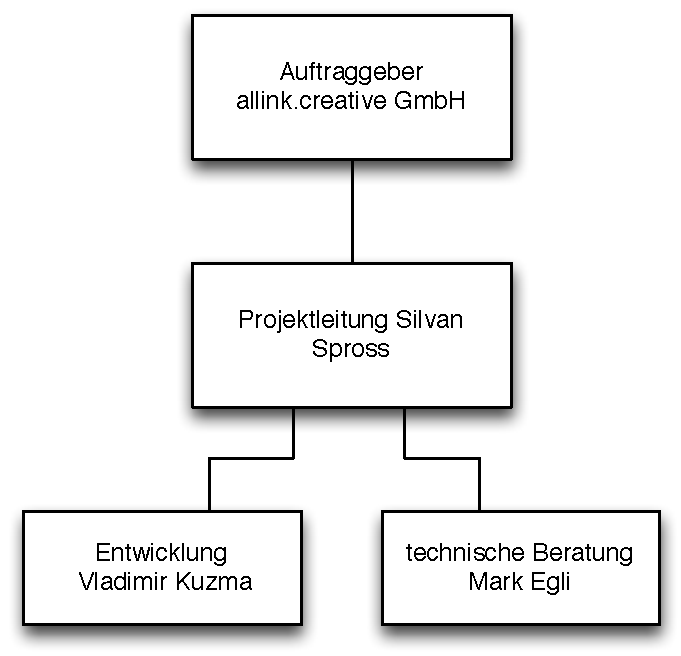
\includegraphics[width=0.5\textwidth,angle=0]{./grafiken/organigram.pdf}
\end{center}
\end{figure}
\footnotetext{Eigene Darstellung}

\section{Projektbeschreibung}
Es soll eine Software in Python erstellt werden, welche kontinuierlich die Qualität von einer konfigurierbaren Menge Django Projekte überprüft. Dazu sollen die Projekte jeweils täglich aus dem Versionierungssystem geklont, Projektspezifische Abhängigkeiten installiert und nach gewissen Anforderungen getestet und abschliessend ein projektübergreifender Report per E-Mail versendet werden.

\section{Rahmenbedingung}
Die Anwendung soll mit folgenden Mitteln realisiert werden:

Technologien
\begin{itemize}
    \item Python 

\end{itemize}

Anwendungen
\begin{itemize}
    \item pep8
    \item pyflakes
    \item jshint
\end{itemize}

Systemen
\begin{itemize}
    \item Mac OS X
    \item Debian lenny
\end{itemize}
    
\section{Systemumgebung}
\begin{itemize}
    \item Betriebsystem (Projekumsetzung): Mac OS X
    \item Editor: vim
    \item Dokumentationshilfsmittel: LaTeX
    \item Entwicklungsumgebung: Python
    \item localer Testserver: Debian Server in einer VM (Virtualbox) 
    \item Versionierung: Git, auf Github veröffentlicht
\end{itemize}

\section{Projektplannungsmethode}
Ich habe mich für die Projektplanungsmethode IPERKA entschieden. \\

\subsection{Begründung}
Für ein kleines Projekt reicht IPERKA meiner Meinung ausreichend aus. Die Planungs- und die Realisierungsphase ist klar getrennt. Es sind alle wichtigen Arbeitsschritte vorhanden, die eine saubere Struktur und ausführliche Dokumentation erlauben. 

\clearpage
